\subsection{Qualität der Skalierung}
Nun wird der Zusammenhang zwischen den verscheiden Skalierungsverfahren und der Qualität der Berechnung gesucht.\\
Es zeigt sich, dass bei der Bestimmung der Parameter das Nearest-Neighbor Verfahren die am genauesten Ergebnisse liefert. Allerdings ist der Wertebereich deutlich eingeschränkt. Die Mindestgröße des Gesichts im Orginal und den geringer Wertebereich bei den Rotationen ist dieses Verfahren eher ungeeignet.\\
Bei dem Linearen-Verfahren ist die Abweichung bei den Rotationen am größten, auch wenn es sich nur um etwa ein halbes Grad handelt. Zwischen dem Bicubic- und Lanczos-Verfahren gibt es in den relevanten Bereichen keinen signifikanten Unterschied, wobei das Lanczos in den kleineren Bereichen gleichmäßigere Ergebnisse. Somit kann die Wahl des Verfahrens vom Rechenaufwand abhängig gemacht werden. 
\subsubsection{Position}
Als erstes wird die berechnete Distanz miteinander verglichen.\\
In \autoref{img_X_Pos_Skal} ist die Abweichung entlang der X-Achse dargestellt. Nearest-Neighbor liefert die genauesten Ergebnisse, auch wenn durch die schlechtere Detektionsrate dieses Verfahren früher ausfällt als die anderen drei.\\
Auf der Y-Achse ist das Lineare-Verfahren etwas besser als die Andren, das Nearest-Neighbor ist hierbei überraschend das Schlechteste, siehe \autoref{img_Y_Pos_Skal}.\\
Nur schwer zu erkennen, da der Unterschied nur minimal ausfällt, ist auch bei der Bestimmung der Z-Position das Nearest-Neighbor-Verfahren am Besten, siehe \autoref{img_Z_Pos_Skal}. Die anderen drei sind nahezu identisch. Bei sehr kleinen Skalierungen existieren durchaus auch sehr große Fehler, diese wurden allerdings bei der Darstellung abgeschnitten, da bei dieser Größe die Detektionsrate so klein ist, dass sie nahezu irrelevant werden.
\begin{figure}
	\centering
	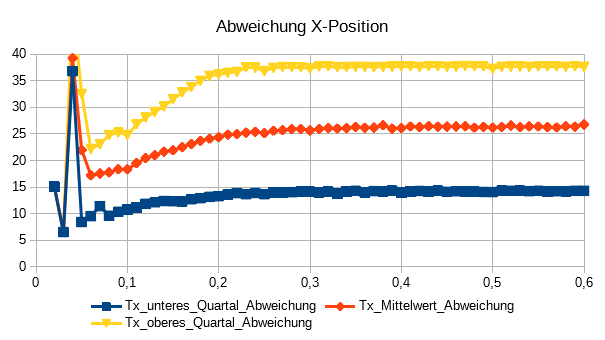
\includegraphics[width=0.45\linewidth]{tabelle2/X_Pos_Cubic}
	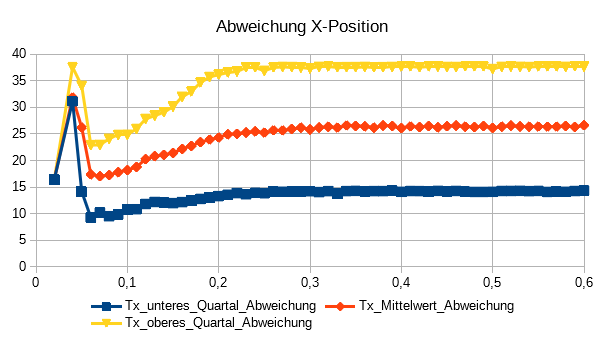
\includegraphics[width=0.45\linewidth]{tabelle2/X_Pos_Lanc}
	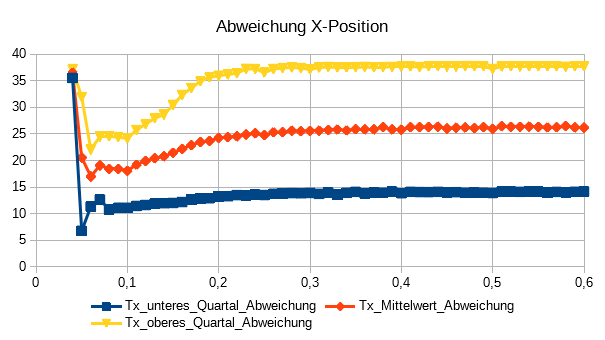
\includegraphics[width=0.45\linewidth]{tabelle2/X_Pos_Linear}
	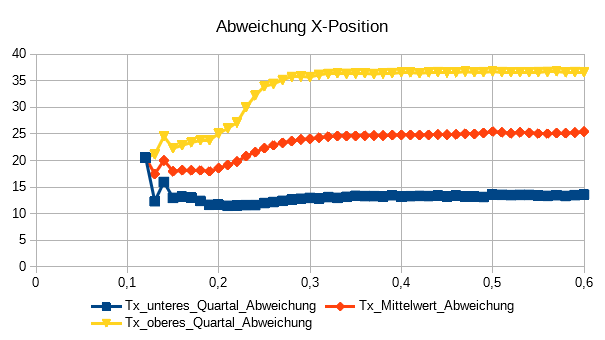
\includegraphics[width=0.45\linewidth]{tabelle2/X_Pos_NN}
	\caption{Zusammenhang zwischen der Skalierung (X-Achse) und der Abweichung in X-Richtung (Y-Achse) in Millimeter. 
	 Bicubic (oben links), Lanczos (oben rechts), Linear (unten links), Nearest-Neighbor (unten rechts)}
	\label{img_X_Pos_Skal}
\end{figure}
\begin{figure}
	\centering
	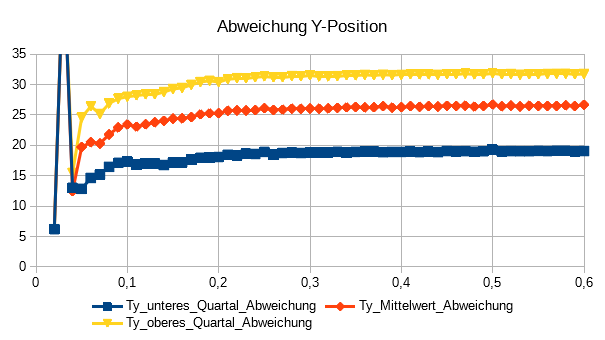
\includegraphics[width=0.45\linewidth]{tabelle2/Y_Pos_Cubic}
	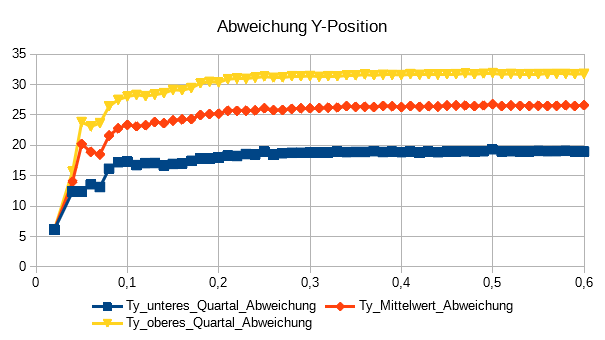
\includegraphics[width=0.45\linewidth]{tabelle2/Y_Pos_Lanc}
	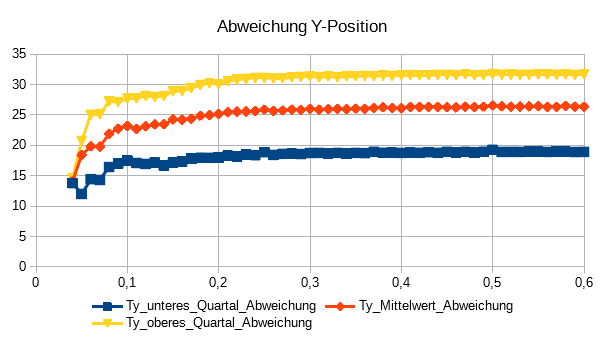
\includegraphics[width=0.45\linewidth]{tabelle2/Y_Pos_Linear}
	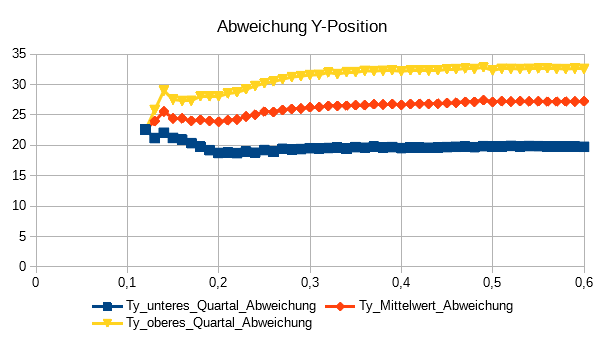
\includegraphics[width=0.45\linewidth]{tabelle2/Y_Pos_NN}
	\caption{Zusammenhang zwischen der Skalierung (X-Achse) und der Abweichung in Y-Richtung (Y-Achse) in Millimeter. 
		Bicubic (oben links), Lanczos (oben rechts), Linear (unten links), Nearest-Neighbor (unten rechts)}
	\label{img_Y_Pos_Skal}
\end{figure}
\begin{figure}
	\centering
	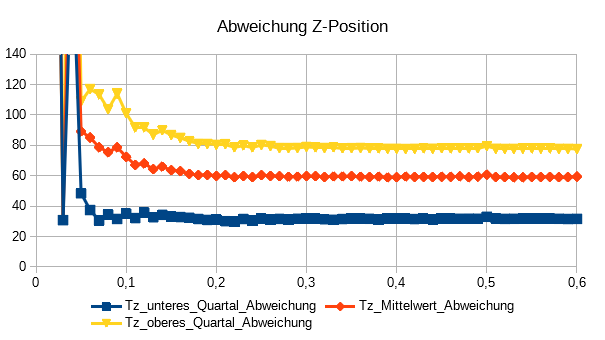
\includegraphics[width=0.45\linewidth]{tabelle2/Z_Pos_Cubic}
	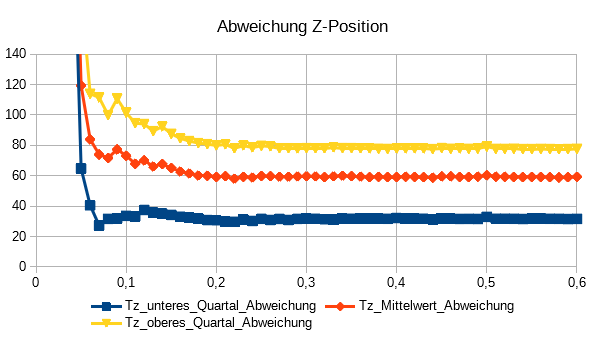
\includegraphics[width=0.45\linewidth]{tabelle2/Z_Pos_Lanc}
	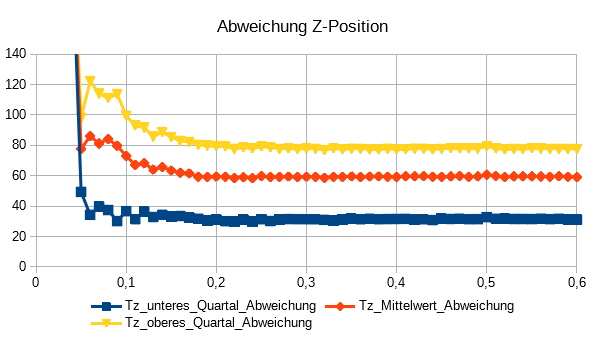
\includegraphics[width=0.45\linewidth]{tabelle2/Z_Pos_Linear}
	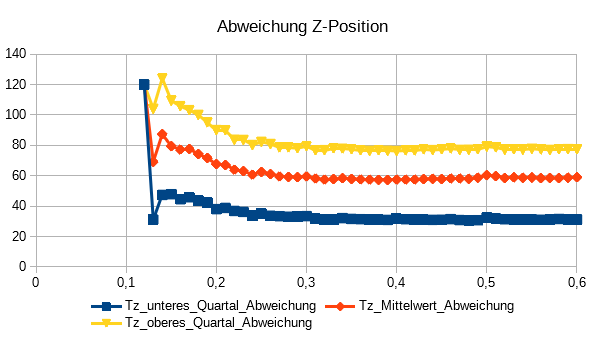
\includegraphics[width=0.45\linewidth]{tabelle2/Z_Pos_NN}
	\caption{Zusammenhang zwischen der Skalierung (X-Achse) und der Abweichung in Z-Richtung (Y-Achse) in Millimeter. 
		Bicubic (oben links), Lanczos (oben rechts), Linear (unten links), Nearest-Neighbor (unten rechts)}
	\label{img_Z_Pos_Skal}
\end{figure}
\subsubsection{Orientierung}
Des weiteren wird der berechneten Winkel um die jeweilige Achse betrachtet und mit den korrekten verglichen. Die geringste Abweichung bei der bestimung der X-Rotation liefert Nearest-Neighbor, siehe \autoref{img_X_Rot_Skal}. Auffällig ist außerdem der kleinere Wertebereich des Linearen-Verfahrens.\\
Auch bei der Y-Rotation schneidet Nearest-Neighbor am besten ab, siehe \autoref{img_Y_Rot_Skal}, allerdings sind die unterscheide minimal.\\
Beider Z-Rotation ist kein erkennbarer Unterschied zwischen den einzelnen Verfahren. Wobei bei Nearest-Neighbor deutlich früher der Wertebereich sinkt.
\begin{figure}
	\centering
	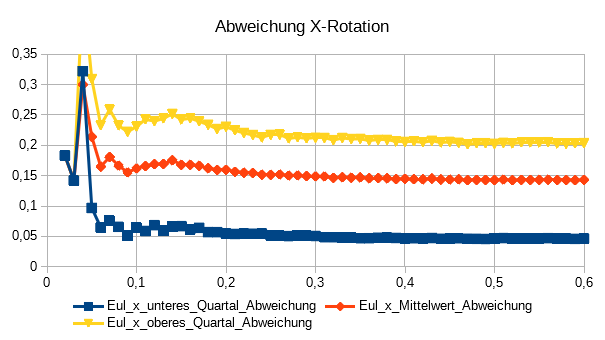
\includegraphics[width=0.45\linewidth]{tabelle2/X_Rot_Cubic}
	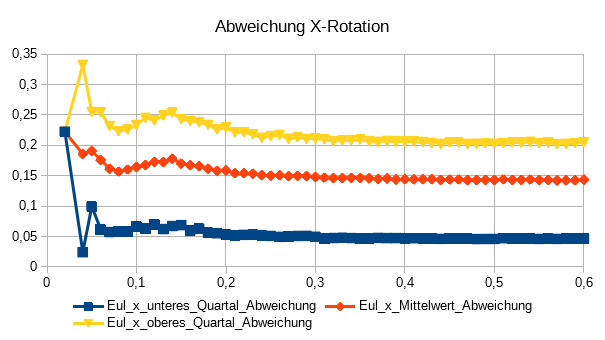
\includegraphics[width=0.45\linewidth]{tabelle2/X_Rot_Lanc}
	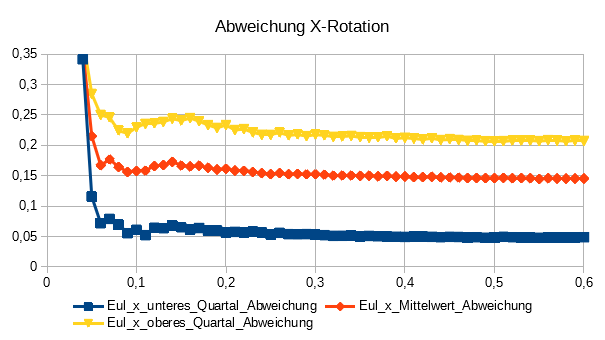
\includegraphics[width=0.45\linewidth]{tabelle2/X_Rot_Linear}
	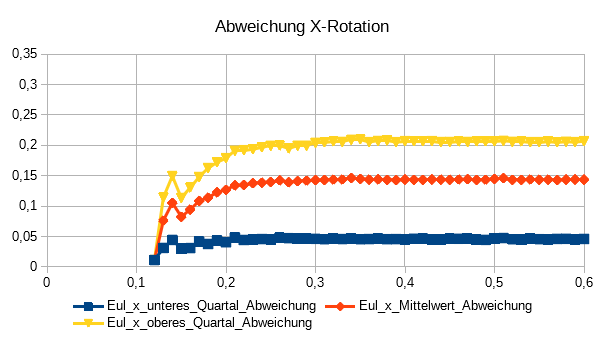
\includegraphics[width=0.45\linewidth]{tabelle2/X_Rot_NN}
	\caption{Zusammenhang zwischen der Skalierung (X-Achse) und der Abweichung des Winkels in X-Richtung, Angabe in Bogenmaß. 
		Bicubic (oben links), Lanczos (oben rechts), Linear (unten links), Nearest-Neighbor (unten rechts)}
	\label{img_X_Rot_Skal}
\end{figure}
\begin{figure}
	\centering
	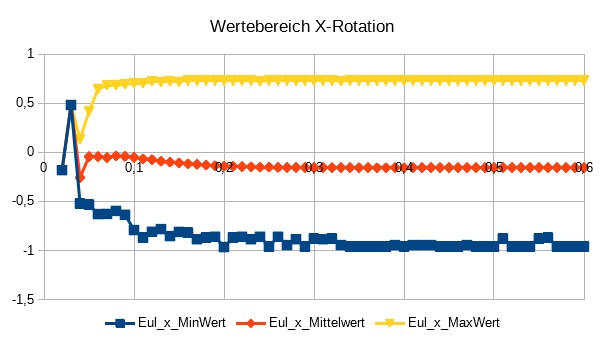
\includegraphics[width=0.45\linewidth]{tabelle2/X_Rot_Val_Cubic}
	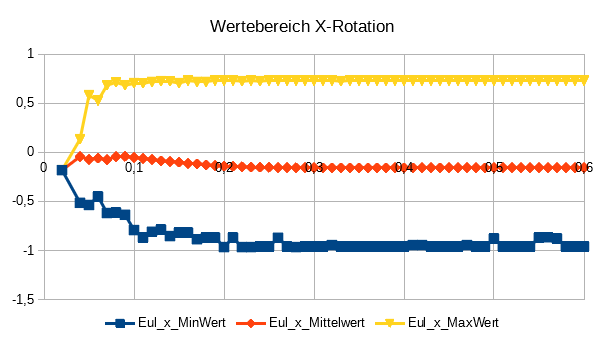
\includegraphics[width=0.45\linewidth]{tabelle2/X_Rot_Val_Lanc}
	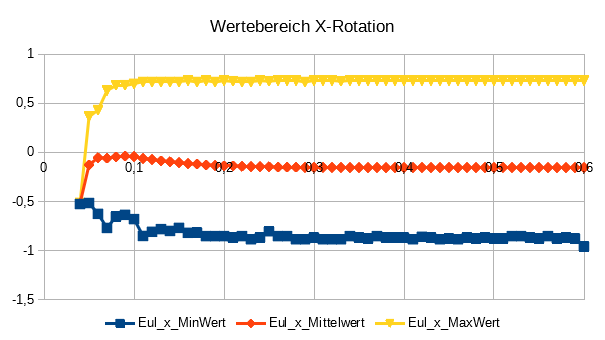
\includegraphics[width=0.45\linewidth]{tabelle2/X_Rot_Val_Linear}
	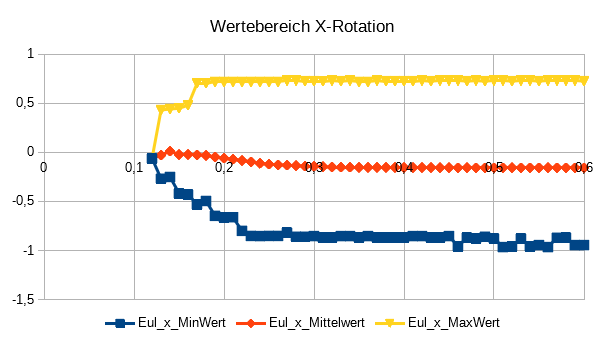
\includegraphics[width=0.45\linewidth]{tabelle2/X_Rot_Val_NN}
	\caption{Zusammenhang zwischen der Skalierung (X-Achse) und der Abweichung des Winkels in X-Richtung, Angabe in Bogenmaß. 
		Bicubic (oben links), Lanczos (oben rechts), Linear (unten links), Nearest-Neighbor (unten rechts)}
	\label{img_X_Rot_Val_Skal}
\end{figure}
\begin{figure}
	\centering
	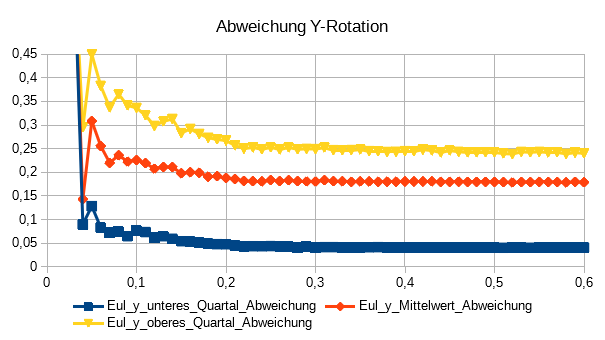
\includegraphics[width=0.45\linewidth]{tabelle2/Y_Rot_Cubic}
	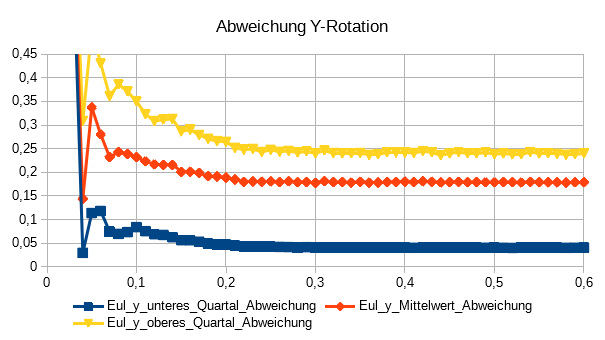
\includegraphics[width=0.45\linewidth]{tabelle2/Y_Rot_Lanc}
	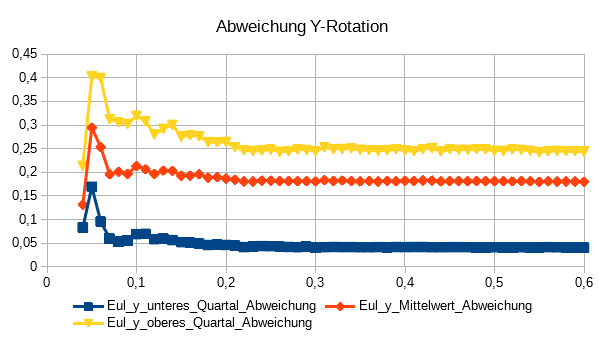
\includegraphics[width=0.45\linewidth]{tabelle2/Y_Rot_Linear}
	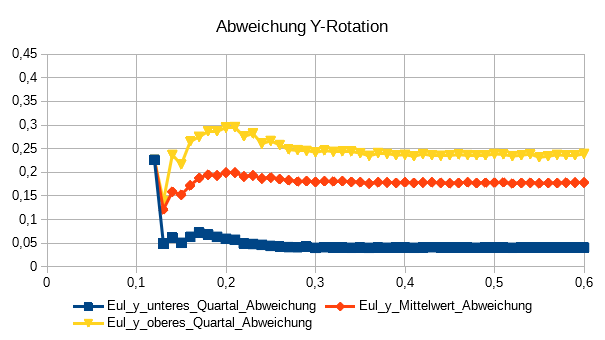
\includegraphics[width=0.45\linewidth]{tabelle2/Y_Rot_NN}
	\caption{Zusammenhang zwischen der Skalierung (X-Achse) und der Abweichung des Winkels in Y-Richtung, Angabe in Bogenmaß.
		Bicubic (oben links), Lanczos (oben rechts), Linear (unten links), Nearest-Neighbor (unten rechts)}
	\label{img_Y_Rot_Skal}
\end{figure}
\begin{figure}
	\centering
	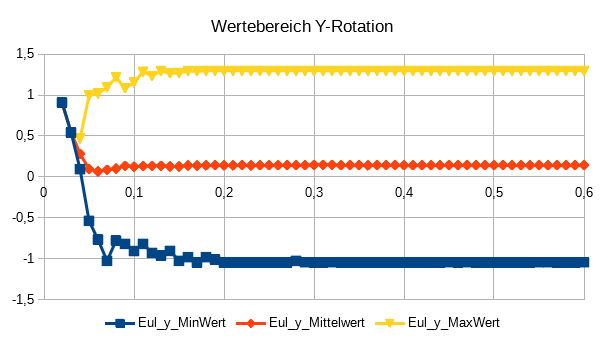
\includegraphics[width=0.45\linewidth]{tabelle2/Y_Rot_Val_Cubic}
	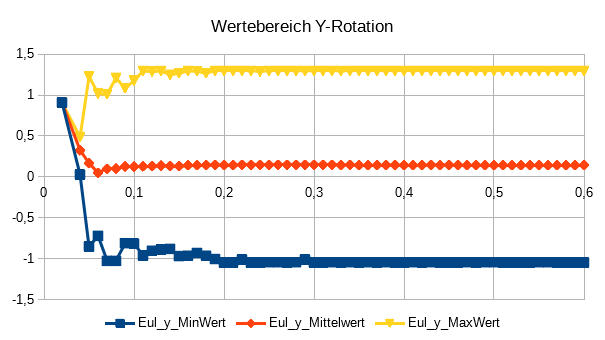
\includegraphics[width=0.45\linewidth]{tabelle2/Y_Rot_Val_Lanc}
	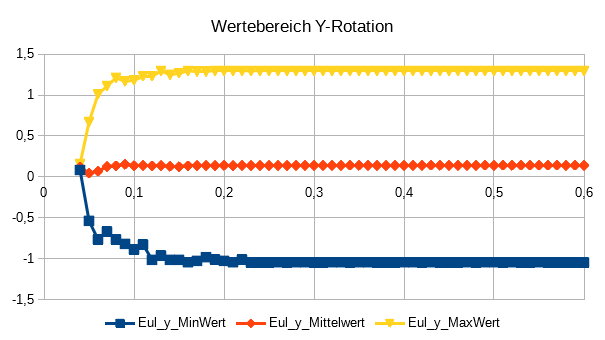
\includegraphics[width=0.45\linewidth]{tabelle2/Y_Rot_Val_Linear}
	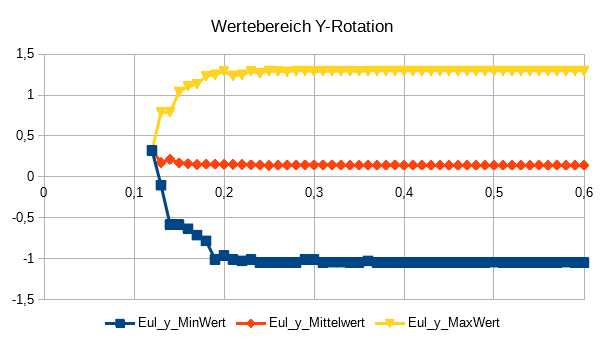
\includegraphics[width=0.45\linewidth]{tabelle2/Y_Rot_Val_NN}
	\caption{Zusammenhang zwischen der Skalierung (X-Achse) und der Wertebereich des Winkels in Y-Richtung, Angabe in Bogenmaß.
		Bicubic (oben links), Lanczos (oben rechts), Linear (unten links), Nearest-Neighbor (unten rechts)}
	\label{img_Y_Rot_Val_Skal}
\end{figure}
\begin{figure}
	\centering
	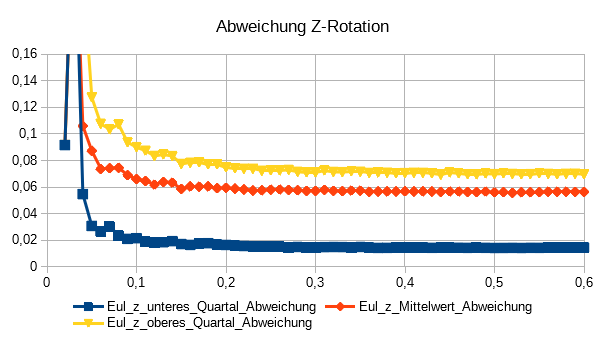
\includegraphics[width=0.45\linewidth]{tabelle2/Z_Rot_Cubic}
	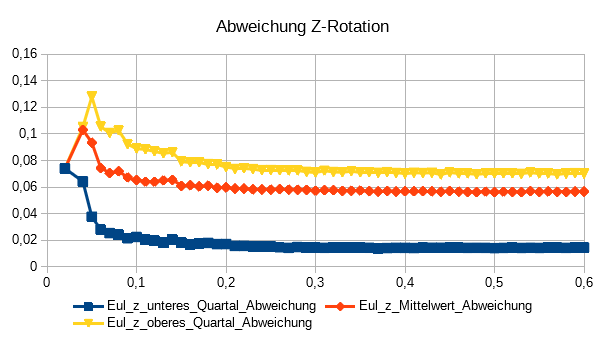
\includegraphics[width=0.45\linewidth]{tabelle2/Z_Rot_Lanc}
	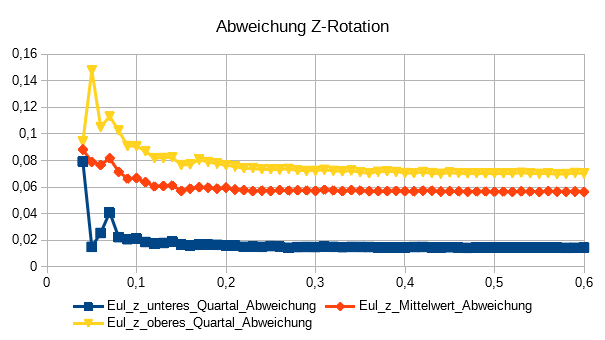
\includegraphics[width=0.45\linewidth]{tabelle2/Z_Rot_Linear}
	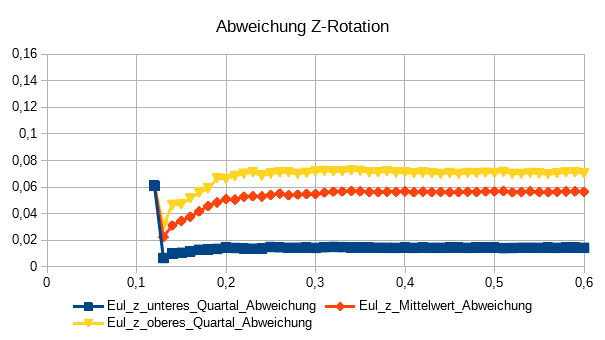
\includegraphics[width=0.45\linewidth]{tabelle2/Z_Rot_NN}
	\caption{Zusammenhang zwischen der Skalierung (X-Achse) und der Abweichung des Winkels in Z-Richtung, Angabe in Bogenmaß.
		Bicubic (oben links), Lanczos (oben rechts), Linear (unten links), Nearest-Neighbor (unten rechts)}
	\label{img_Z_Rot_Skal}
\end{figure}
\begin{figure}
	\centering
	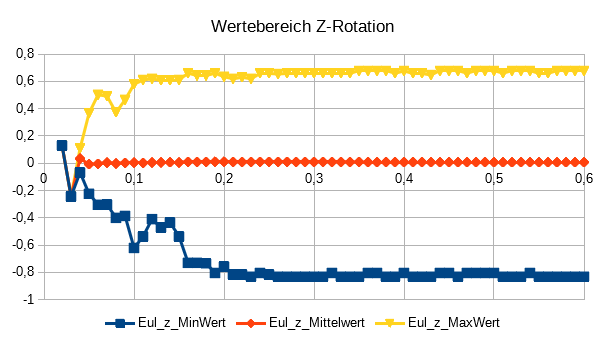
\includegraphics[width=0.45\linewidth]{tabelle2/Z_Rot_Val_Cubic}
	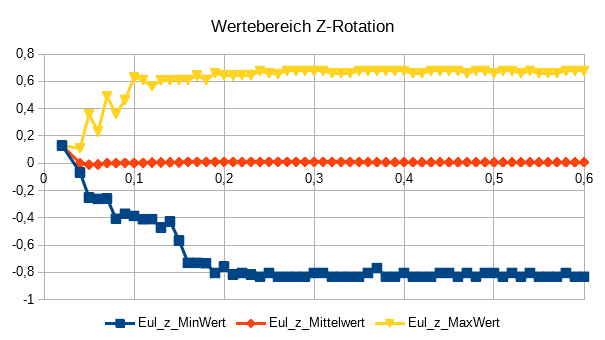
\includegraphics[width=0.45\linewidth]{tabelle2/Z_Rot_Val_Lanc}
	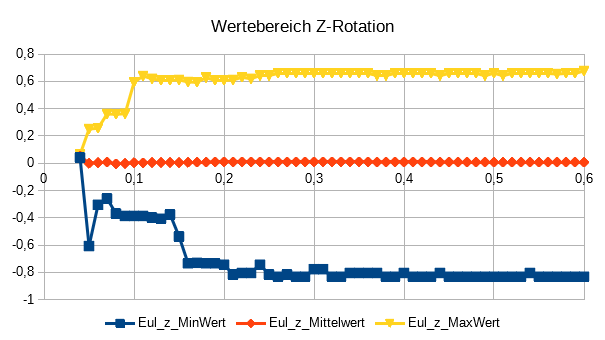
\includegraphics[width=0.45\linewidth]{tabelle2/Z_Rot_Val_Linear}
	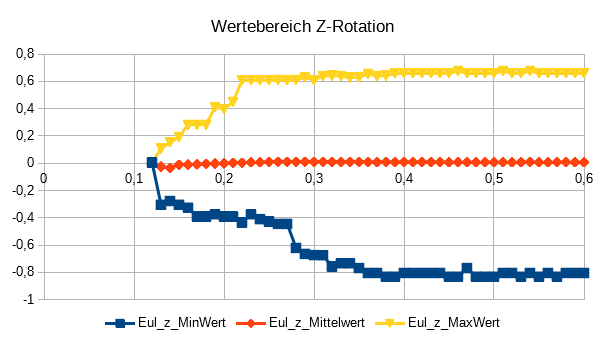
\includegraphics[width=0.45\linewidth]{tabelle2/Z_Rot_Val_NN}
	\caption{Zusammenhang zwischen der Skalierung (X-Achse) und der Wertebereiche des Winkels in Z-Richtung, Angabe in Bogenmaß.
		Bicubic (oben links), Lanczos (oben rechts), Linear (unten links), Nearest-Neighbor (unten rechts)}
	\label{img_Z_Rot_Val_Skal}
\end{figure}